\documentclass[a4paper]{article}

%% Language and font encodings
\usepackage[english]{babel}
\usepackage[utf8x]{inputenc}
\usepackage[T1]{fontenc}

%% Sets page size and margins
\usepackage[a4paper,top=3cm,bottom=2cm,left=3cm,right=3cm,marginparwidth=1.75cm]{geometry}

%% Useful packages
\usepackage{amsmath}
\usepackage{graphicx}
\usepackage[colorinlistoftodos]{todonotes}
\usepackage[colorlinks=true, allcolors=blue]{hyperref}

\title{Actividad 6}
\author{Isaac Neri Gómez Sarmiento}
\date{27 de marzo, 2018}
\begin{document}
\maketitle


\section{Introducción}
En esta actividad, analizamos el movimiento de 2 resortes acoplados, es decir 2 resortes y 2 pesos conectados en serie colgando de un techo. Se utilizó el artículo \textit{Coupled spring equations} de Temple H. Fay y Sarah Duncan para obtener las soluciones a las ecuaciones diferenciales que se construyen para modelar el sistema. Estas soluciones son funciones de desplazamiento que dependen del tiempo. 

Se analizaron 4 casos en donde se conocen parámetros como las constantes de los resortes, masas, longitudes naturales, desplazamientos y velocidades iniciales. Las soluciones exactas se proporcionan en los 2 primeros casos, pero no en los 2 últimos casos. En todos los casos se determinaron soluciones numéricas usando la biblioteca de python \textbf{scipy.integrate}, específicamente la función \textbf{odeint}.

\section{Modelo de resortes acoplados}
La siguiente imágen representa gráficamente el sistema de resortes acoplados.

\begin{figure}[ht!]
\centering
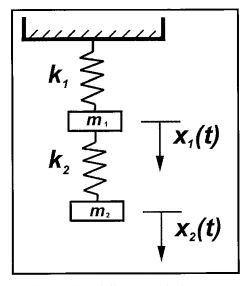
\includegraphics[width=0.3\textwidth]{Resortes_acoplados.JPG}
\caption{\label{fig:Sistema de resortes acoplados}Sistema de resortes acoplados}
\end{figure}

Se tiene un resorte cuya constante es $k_1$ y éste está colgando de un techo. En la parte inferior del resorte se encuentra una masa $m_1$, de donde cuelga un resorte con constante $k_2$. En la parte inferior del segundo resorte cuelga una pesa de masa $m_2$. Se le permite al sistema llegar al reposo en equilibrio para poder medir apartir de ahí los posteriores desplazamientos de los centros de masa de cada pesa, los cuales se denotan como $x_1(t)$ y $x_2(t)$.

Las ecuaciones diferenciales se obtuvieron a partir de una sumatoria de fuerzas.


\begin{figure}[ht!]
\centering
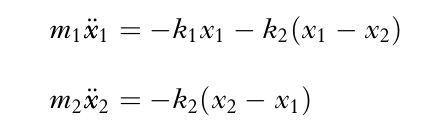
\includegraphics[width=0.3\textwidth]{Ecuacion2_1.png}
\caption{\label{fig:Sistema de resortes acoplados}Sumatoria de fuerzas en cada resorte}
\end{figure}

\newpage
De esta manera obtenemos un par de ecuaciones diferenciales de segundo orden. Para encontrar una ecuación para $x_1$ que no involucre $x_2$, despejamos a $x_2$, obteniendo:


\begin{figure}[ht!]
\centering
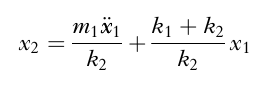
\includegraphics[width=0.3\textwidth]{Ecuacion2_2.png}
%\caption{\label{fig:Sistema de resortes acoplados}Sumatoria de fuerzas en cada resorte}
\end{figure}

Sustituyendo $x_2$ en la segunda ecuación diferencial, y simplificando, obtenemos:


\begin{figure}[ht!]
\centering
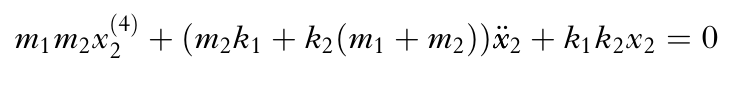
\includegraphics[width=0.5\textwidth]{Ecuacion2_3.png}
%\caption{\label{fig:Sistema de resortes acoplados}Sumatoria de fuerzas en cada resorte}
\end{figure}

Por lo tanto el movimiento de la primera pesa está determinado por esta ecuación diferencial lineal de cuarto orden.
Para encontrar una ecuación que solo involucre $x_2$, despejamos a $x_1$ de la segunda ecuación diferencial original:

\begin{figure}[ht!]
\centering
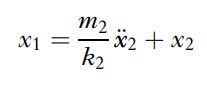
\includegraphics[width=0.2\textwidth]{Ecuacion_2_4.JPG}
%\caption{\label{fig:Sistema de resortes acoplados}Sumatoria de fuerzas en cada resorte}
\end{figure}

y sustituimos en la primera ecuación diferencial original, produciendo la ecuación:


\begin{figure}[ht!]
\centering
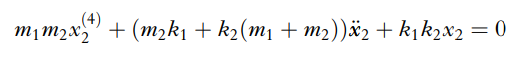
\includegraphics[width=0.5\textwidth]{Ecuacion2_5.PNG}
%\caption{\label{fig:Sistema de resortes acoplados}Sumatoria de fuerzas en cada resorte}
\end{figure}

Podemos ver que tiene la misma estructura que la ecuación que describe al primer resorte. 

Si consideramos que las masas valen 1 kg de cada pesa, podemos simplificar la ecuación y determinar la ecuación característica que nos permite obtener las soluciones para $x_1(t)$ y $x_2(t)$.

\begin{figure}[ht!]
\centering
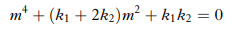
\includegraphics[width=0.4\textwidth]{ecuacion_caracteristica.PNG}
%\caption{\label{fig:Sistema de resortes acoplados}Sumatoria de fuerzas en cada resorte}
\end{figure}

cuyas raíces son:

\begin{figure}[ht!]
\centering
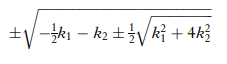
\includegraphics[width=0.3\textwidth]{roots.PNG}
%\caption{\label{fig:Sistema de resortes acoplados}Sumatoria de fuerzas en cada resorte}
\end{figure}

\subsection{Ejemplo 2.1}
Describir el movimiento para las constantes de los resortes $k1=6$ y $k2=4$ con condiciones iniciales:

\begin{figure}[ht!]
\centering
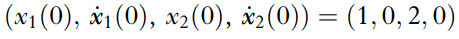
\includegraphics[width=0.5\textwidth]{Ejemplo2_1.PNG}
%\caption{\label{fig:Sistema de resortes acoplados}Sumatoria de fuerzas en cada resorte}
\end{figure}



En general se utilizó el mismo código para resolver los 4 ejemplos, solo que con algunas modificaciones en los parámetros, según el caso.

Primeramente, se define la función vectorfield que define las ecuaciones diferenciales para el sistema de resortes acoplados. \\

Las entradas son: w, t, p
\begin{itemize}

\item \textbf{w} es el vector que contiene las variables de posición (xi), y las de velocidad (vi) para cada uno de los resortes. 
\item \textbf{t} es el tiempo
\item \textbf{p} es el vector que contiene los parámetros como la masa, la constante de los resortes, longitudes iniciales y constantes de amortiguamiento.

\end{itemize}

\begin{verbatim}
def vectorfield(w, t, p):
    x1, y1, x2, y2 = w
    m1, m2, k1, k2, L1, L2, b1, b2 = p

    f = [y1,
         (-b1 * y1 - k1 * (x1) + k2 * (x2 - x1)) / m1,
         y2,
         (-b2 * y2 - k2 * (x2 - x1)) / m2]
    return f
\end{verbatim}

Se importan las bibliotecas numpy y scipy. De la biblioteca scipy se importa la función "odeint" para resolver las ecuaciones diferenciales.

\begin{verbatim}

from scipy.integrate import odeint
import numpy as np

# Parameter values
# Masses:
m1 = 1.0
m2 = 1.0
# Spring constants
k1 = 6.0
k2 = 4.0
# Natural lengths
L1 = 0.0
L2 = 0.0
# Friction coefficients
b1 = 0.0
b2 = 0.0

# Initial conditions
# x1 and x2 are the initial displacements; y1 and y2 are the initial velocities
x1 = 1.0
y1 = 0.0
x2 = 2.0
y2 = 0.0

# ODE solver parameters
abserr = 1.0e-8
relerr = 1.0e-6
stoptime = 25
numpoints = 500

# Create the time samples for the output of the ODE solver.

t = [stoptime * float(i) / (numpoints - 1) for i in range(numpoints)]

# Pack up the parameters and initial conditions:
p = [m1, m2, k1, k2, L1, L2, b1, b2]
w0 = [x1, y1, x2, y2]

# Call the ODE solver.
wsol = odeint(vectorfield, w0, t, args=(p,),
              atol=abserr, rtol=relerr)

with open('two_springs1.dat', 'w') as f: # Print & save the solution. 
 for t1, w1 in zip(t, wsol): print(t1, w1[0], w1[1], w1[2],w1[3],
  np.abs((w1[0]-(np.cos(np.sqrt(2)*t1)))/(np.cos(np.sqrt(2)*t1))), 
  np.abs((w1[2]-(2*np.cos(np.sqrt(2)*t1)))/(2*np.cos(np.sqrt(2)*t1))), file=f)
  
\end{verbatim}

Al haber resuelto la ecuación, se procedió a graficar los desplazamientos x1 y x2 contra el tiempo y los phase portraits para x1 y x2.

\begin{figure}[h!]
\centering 
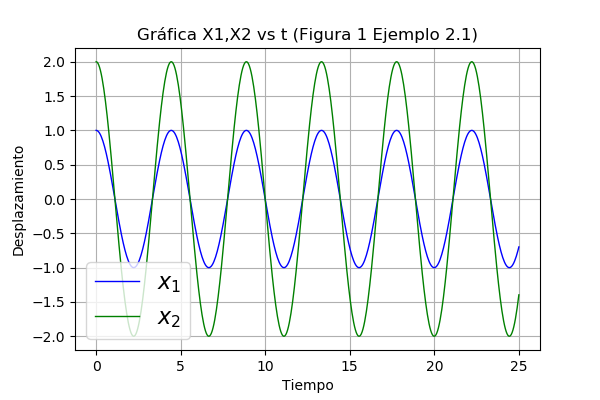
\includegraphics[width=60mm]{Figura1Ex2_1.png}
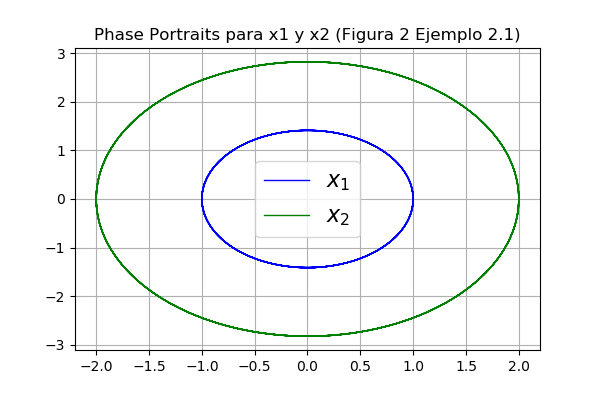
\includegraphics[width=60mm]{Figura2Ex2_1.png}
\end{figure}

La solución analítica que se obtuvo en el artículo está dada por


\begin{center}
$x_1(t)=\cos\sqrt[]{2}t$

$x_2(t)=2\cos\sqrt[]{2}t$
\end{center}

La gráfica del error relativo entre la solución aproximada y la solución exacta es la siguiente:

\begin{figure}[ht!]
\centering
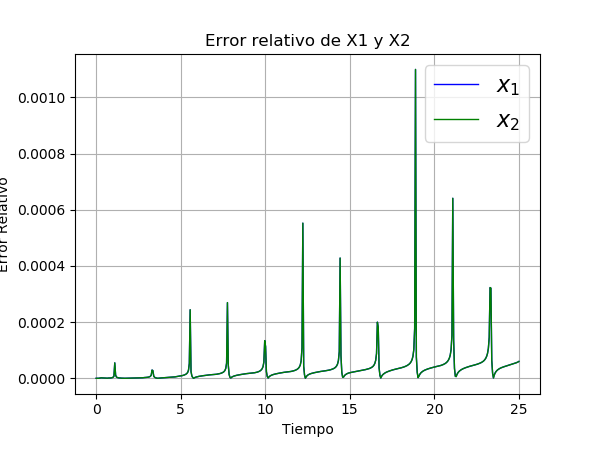
\includegraphics[width=0.5\textwidth]{ErrorEx2_1.png}
\end{figure}

\subsection{Ejemplo 2.2}
Describa el movimiento para las constantes de resorte $k_1=6$ y $k_2=4$ con las condiciones iniciales:

\begin{figure}[ht!]
\centering
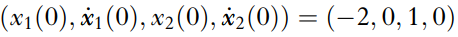
\includegraphics[width=0.5\textwidth]{Ejemplo2_2.PNG}
\end{figure}

A continuación se muestra el segmento de código que se cambió del código anterior:

\begin{verbatim}

from scipy.integrate import odeint
import numpy as np

# Parameter values
# Masses:
m1 = 1.0
m2 = 1.0
# Spring constants
k1 = 6.0
k2 = 4.0
# Natural lengths
L1 = 0.0
L2 = 0.0
# Friction coefficients
b1 = 0.0
b2 = 0.0

# Initial conditions
# x1 and x2 are the initial displacements; y1 and y2 are the initial velocities
x1 = -2.0
y1 = 0.0
x2 = 1.0
y2 = 0.0

# ODE solver parameters
abserr = 1.0e-8
relerr = 1.0e-6
stoptime = 25
numpoints = 500

# Create the time samples for the output of the ODE solver.

t = [stoptime * float(i) / (numpoints - 1) for i in range(numpoints)]

# Pack up the parameters and initial conditions:
p = [m1, m2, k1, k2, L1, L2, b1, b2]
w0 = [x1, y1, x2, y2]

# Call the ODE solver.
wsol = odeint(vectorfield, w0, t, args=(p,),
              atol=abserr, rtol=relerr)

with open('two_springs2.dat', 'w') as f: # Print & save the solution. 
 for t1, w1 in zip(t, wsol): print(t1, w1[0], w1[1], w1[2], w1[3],
 np.abs((w1[0]-(-2*np.cos(2*np.sqrt(3)*t1)))/(-2*np.cos(2*np.sqrt(3)*t1))), 
 np.abs((w1[2]-(np.cos(2*np.sqrt(3)*t1)))/(np.cos(2*np.sqrt(3)*t1))), file=f)
  
\end{verbatim}

Las gráficas resultantes son las siguientes:
\begin{figure}[ht!]
\centering 
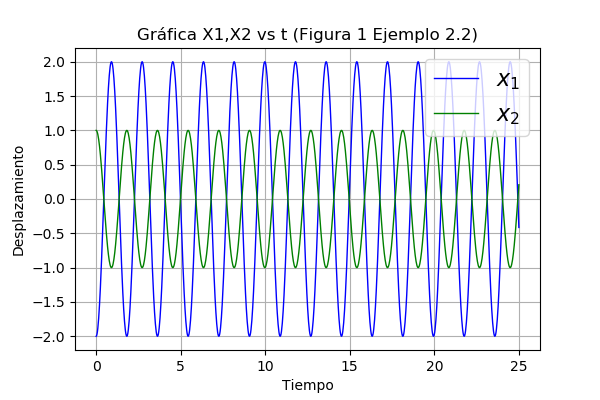
\includegraphics[width=60mm]{Figura1Ex2_2.png}
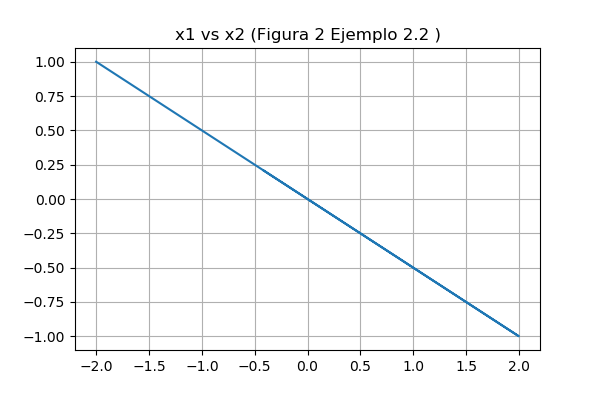
\includegraphics[width=60mm]{Figura2Ex2_2.png}
\end{figure}

La solución analítica está determinada por:
\begin{center}
$x_1(t)=-2\cos2\sqrt[]{3}t$

$x_2(t)=\cos2\sqrt[]{3}t$
\end{center}


La gráfica del error relativo de la solución analítica y la solución aproximada es la siguiente:

\begin{figure}[ht!]
\centering 
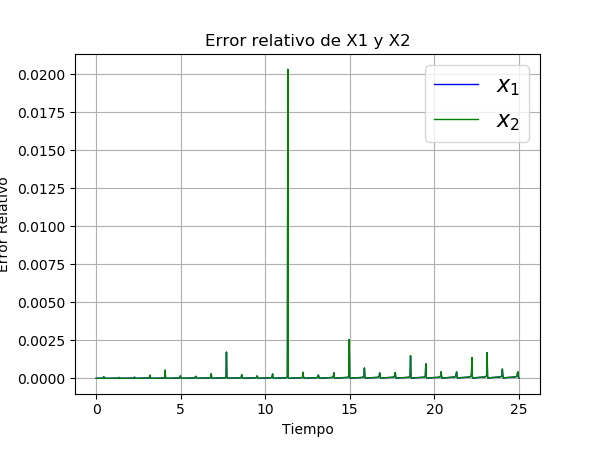
\includegraphics[width=70mm]{ErrorEx2_2.png}
\end{figure}

\newpage
\subsection{Ejemplo 2.3}
Describa el movimiento para las constantes de resprte $k_1=0.4$ y $k_2=1.808$ con las siguientes condiciones iniciales:

\begin{figure}[ht!]
\centering
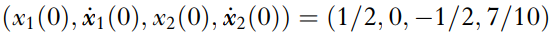
\includegraphics[width=70mm]{Ejemplo2_3.PNG}
\end{figure}

En este ejemplo y en el siguiente no se proporcionan las soluciones analíticas de las ecuaciones diferenciales, por lo que no se obtuvo una gráfica para el error relativo.

El segmento de código que fue modificado quedó de la siguiente manera:

\begin{verbatim}

from scipy.integrate import odeint
import numpy as np

# Parameter values
# Masses:
m1 = 1.0
m2 = 1.0
# Spring constants
k1 = 0.4
k2 = 1.808
# Natural lengths
L1 = 0.0
L2 = 0.0
# Friction coefficients
b1 = 0.0
b2 = 0.0

# Initial conditions
# x1 and x2 are the initial displacements; y1 and y2 are the initial velocities
x1 = 1./2.
y1 = 0.0
x2 = -1./2.
y2 = 7./10.

# ODE solver parameters
abserr = 1.0e-8
relerr = 1.0e-6
stoptime = 50
numpoints = 800

# Create the time samples for the output of the ODE solver.

t = [stoptime * float(i) / (numpoints - 1) for i in range(numpoints)]

# Pack up the parameters and initial conditions:
p = [m1, m2, k1, k2, L1, L2, b1, b2]
w0 = [x1, y1, x2, y2]

# Call the ODE solver.
wsol = odeint(vectorfield, w0, t, args=(p,),
              atol=abserr, rtol=relerr)

with open('two_springs3.dat', 'w') as f:
  # Print & save the solution.
  for t1, w1 in zip(t, wsol):
  print(t1, w1[0], w1[1], w1[2], w1[3], file=f)
 
\end{verbatim}


Las gráficas que se obtuvieron son las siguientes:

\begin{figure}[ht!]
\centering 
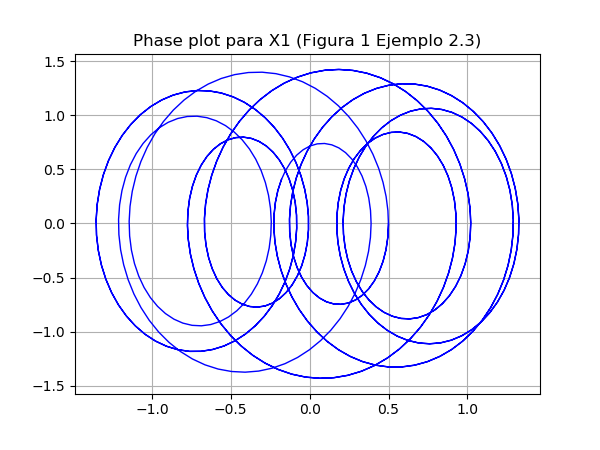
\includegraphics[width=65mm]{Figura1Ex2_3.png}
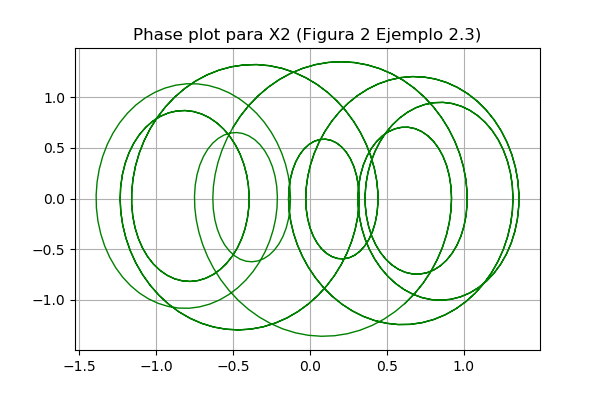
\includegraphics[width=70mm]{Figura2Ex2_3.png}
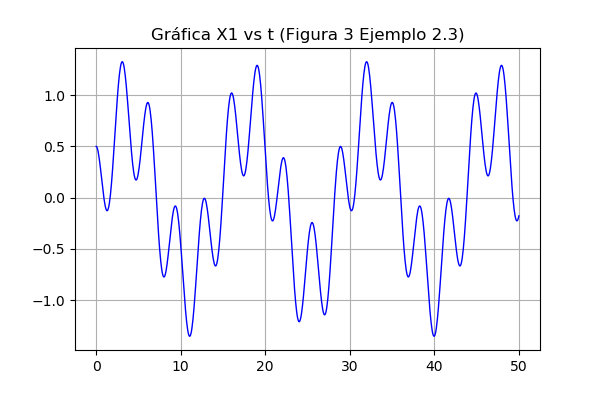
\includegraphics[width=70mm]{Figura3Ex2_3.png}
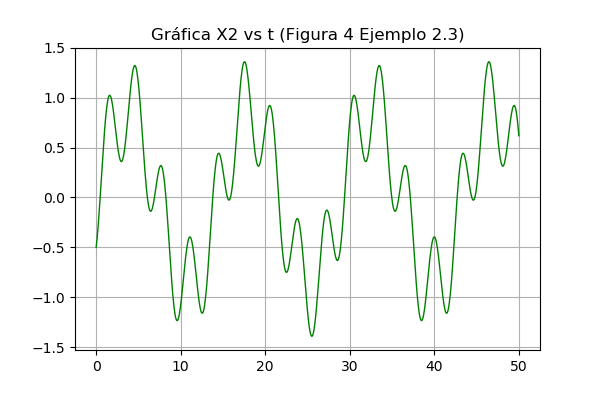
\includegraphics[width=70mm]{Figura4Ex2_3.png}
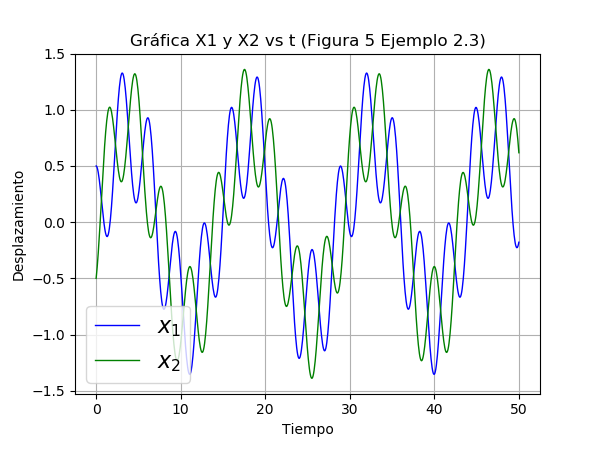
\includegraphics[width=70mm]{Figura5Ex2_3.png}
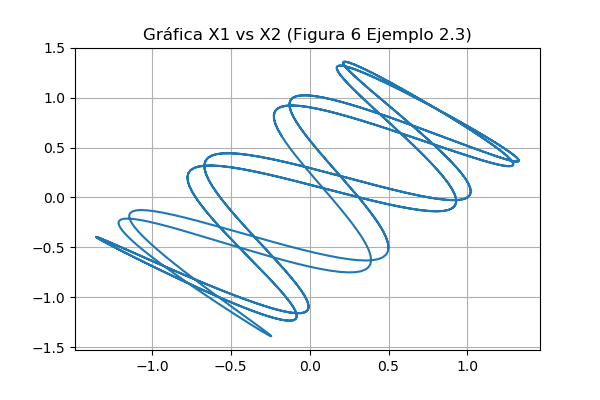
\includegraphics[width=70mm]{Figura6Ex2_3.png}
\end{figure}


\newpage
\subsection{Ejemplo 2.4}
Asuma que $m_1=m_2=1$. Describa el movimineto para las constantes de resorte $k_1=0.7$ y $k_2=1.808$, coeficientes de amortiguamiento $b_1=0.1$ y $b_2=0.2$, con las condiciones iniciales:

\begin{figure}[ht!]
\centering 
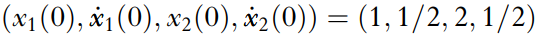
\includegraphics[width=70mm]{Ejemplo2_4.PNG}
\end{figure}

La diferencia entre este ejemplo y los anteriores, es que ahora se toman en cuenta los coeficientes de amortiguamiento.

El segmento de código queda como sigue:

\begin{verbatim}
# Use ODEINT to solve the differential equations defined by the vector field
from scipy.integrate import odeint

# Parameter values
# Masses:
m1 = 1.0
m2 = 1.0
# Spring constants
k1 = 0.4
k2 = 1.808
# Natural lengths
L1 = 0.0
L2 = 0.0
# Friction coefficients
b1 = 0.1
b2 = 0.2

# Initial conditions
# x1 and x2 are the initial displacements; y1 and y2 are the initial velocities
x1 = 1
y1 = 1./2.
x2 = 2.
y2 = 1./2.

# ODE solver parameters
abserr = 1.0e-8
relerr = 1.0e-6
stoptime = 50
numpoints = 800

# Create the time samples for the output of the ODE solver.
# I use a large number of points, only because I want to make
# a plot of the solution that looks nice.
t = [stoptime * float(i) / (numpoints - 1) for i in range(numpoints)]

# Pack up the parameters and initial conditions:
p = [m1, m2, k1, k2, L1, L2, b1, b2]
w0 = [x1, y1, x2, y2]

# Call the ODE solver.
wsol = odeint(vectorfield, w0, t, args=(p,),
              atol=abserr, rtol=relerr)

with open('two_springs4.dat', 'w') as f:
  # Print & save the solution.
  for t1, w1 in zip(t, wsol):
  print(t1, w1[0], w1[1], w1[2], w1[3], file=f)
\end{verbatim}


\newpage
Se presentan las gráficas obtenidas:
\begin{figure}[ht!]
\centering 
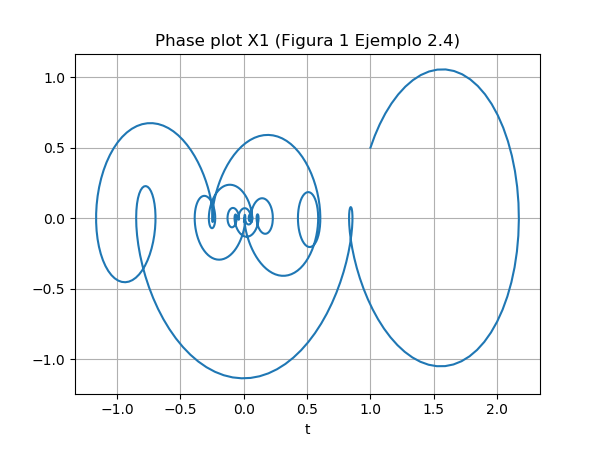
\includegraphics[width=65mm]{Figura1Ex2_4.png}
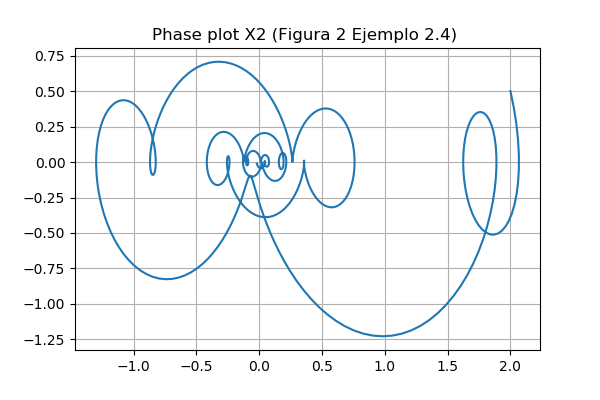
\includegraphics[width=70mm]{Figura2Ex2_4.png}
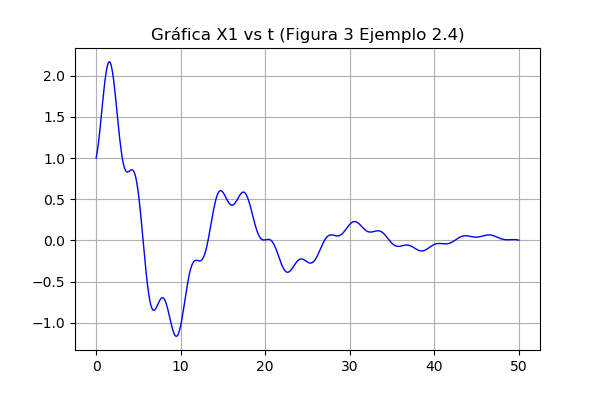
\includegraphics[width=70mm]{Figura3Ex2_4.png}
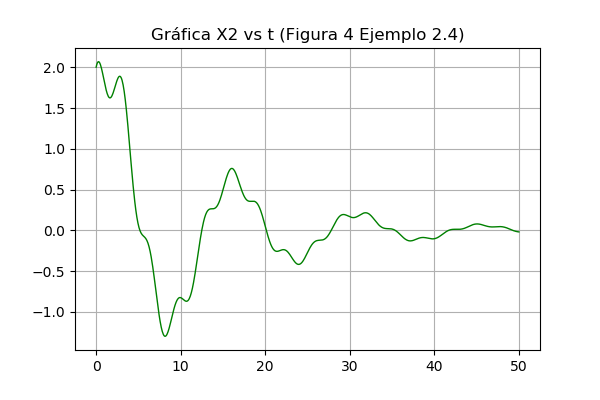
\includegraphics[width=70mm]{Figura4Ex2_4.png}
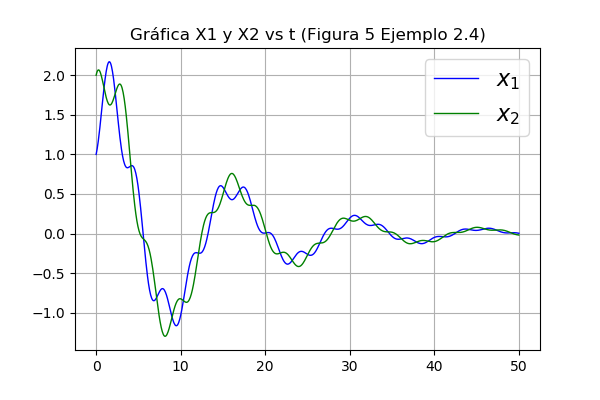
\includegraphics[width=70mm]{Figura5Ex2_4.png}
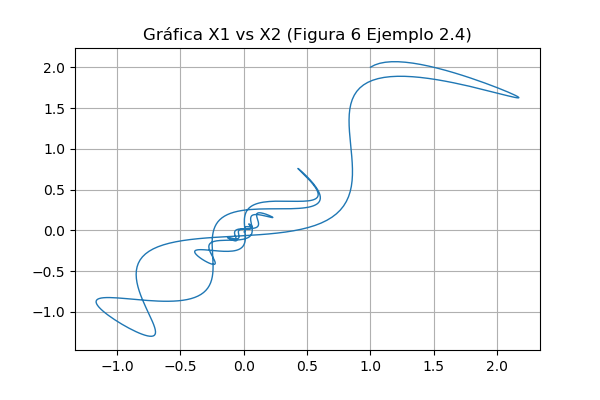
\includegraphics[width=70mm]{Figura6Ex2_4.png}
\end{figure}


\section{Conclusión}

Esta actividad fue un primer acercamiento al modelado de un sistema físico, sistema de resortes acoplados,  usando la ayuda de algoritmos computacionales para resolver ecuaciones diferenciales ordinarias. 

Algunas observaciones se pudieron rescatar, como el hecho de que entre más parámetros se tomen en cuenta (como las constantes de amortiguamiento en el último ejemplo), más caótico se vuelve el movimiento y se ve reflejado en la simetría de las gráficas. Los errores relativos representados en gráficas en los dos primeros ejemplos, muestran que no hay mucha diferencia entre la solución analítica y la aproximada, siendo la máxima diferencia no más del 2\%.

\section{Apéndice}

\begin{enumerate}
\item \textbf {¿En general te pareció interesante esta actividad de modelación matemática? ¿Qué te gustó mas? ¿Qué no te gustó?}


Si me pareció interesante, en especial que la solución aproximada haya sido muy fiel a la analítica. Me llama la atención la forma de las gráficas. No hubo nada que no me gustara, lo único que no entendí fue la interpretación de la gráficas \textit{phaseplot}.

\item \textbf {La cantidad de material te pareció ¿bien?, ¿suficiente?, ¿demasiado?}

Me pareció suficiente, ya que no tuvimos que resumir mucho texto y además, que estamos familiarizados con el tema. 

\item \textbf {¿Cuál es tu primera impresión de Jupyter Lab? }

Es muy similar a Jupyter Notebook, con la diferencia que se pueden acomodar las celdas en el orden que uno quiere después de haberlas creado o se puede acceder fácilmente a las imágenes o archivos guardados.

\item \textbf {Respecto al uso de funciones de SciPy, ¿ya habías visto integración numérica en tus cursos anteriores? ¿Cuál es tu experiencia?.}

Si había visto otros métodos de integración numérica. En cálculo 2 y Fortran ví el método de los trapecios. En análisis numérico, además del de trapecios, vi el de Simpson 1/3 y 3/8. 

Para programar, el de trapecios es más fácil, ya que en el de Simpson debes considerar casos en el que debes usar 1/3 y 3/8 dependiendo del número de particiones.


\item \textbf {El tema de sistema de masas acopladas con resortes, ¿ya lo habías resuelto en tu curso de Mecánica 2?  }

No que yo recuerde. Solo para un sistema de masas con un solo resorte. 


\item \textbf {¿Qué le quitarías o agregarías a esta actividad para hacerla más interesante y divertida?  }

Habría sido mejor Que hubiera consistido en un solo problema, en el cual por equipos hubieramos obtenido experimentalmente las condiciones iniciales, las masas, las constantes de los resortes y los coeficientes de amortiguamiento. De esta manera, proseguiriamos a obtener nosotros las soluciones analíticas a las ecuaciones diferenciales y por último la solución con integración numérica. 


\end{enumerate}




\section{Bibliografía}

\noindent
Temple H. Fay and Sarah D. Graham. Coupled Spring Equations. Recuperado el 12 de Marzo 2018 de: \url{http://math.oregonstate.edu/~gibsonn/Teaching/MTH323-010S15/Supplements/coupled_spring.pdf}

Sci-py Cookbook. Coupled spring-mass system. Recuperado el 12 de Marzo 2018 de: \url {http://scipy-cookbook.readthedocs.io/items/CoupledSpringMassSystem.html}

\end{document}